\chapter{RESULTS AND DISCUSSION}
The outputs of  {\bf HydRA} program are compared against the output of the \newline 
software MDLHydroD. The development of the 
MDLHydroD software is explained in \cite{guha2013development} and \cite{guha2015estimation}.
For comparison KCS and KVLCC2 vessels' hull structure is used. 

\section{Forward speed comparisons for KCS Vessel}
KCS ( Krisco container ship ) is a fine form container ship and its particulars are listed in Table 
\ref{tab:kcs_principal_particulars}. 
For comparison, frequencies are used from
$-0.03$ with $+0.03$ increment and in totoal $34$ frequencies are used. Ship's speed is $8\,\si{m.s^{-1}}$. 
Incident angles used 
ranges from $0^{\circ}$ to $345^{\circ}$ with $15^{\circ}$ increment. Simulation is ran for 6 modes of motion.  
The comparison of added mass for different angles are shown in figure \ref{fig:kcs_addedmass_1}.
Comparisons of radiation damping is shown in figure \ref{fig:radition_damp_125}. 
Comparisons of Froude Krylov force is shown in figure \ref{fig:kcs_froude_krylov}.
Comparisons of Scattering force is shown in figure \ref{fig:kcs_scattering_135}. 
Comparisons of RAO is shown in figure \ref{fig:kcs_rao_120}
and figure \ref{fig:kcs_rao_135}

\begin{table}[h]
    \centering
    \setlength{\tabcolsep}{10pt} % Default value: 6pt
    \renewcommand{\arraystretch}{1.17} % Default value: 1
    \begin{tabular}{|c|c|}
        \hline
        {\bf Main Particulars} & {\bf Value} \\
        \hline 
        Length between perpendiculars $L ~(m)$ & 230 \\ 
        Breadth $B ~(m)$ & 32.2  \\
        Draft $d ~(m)$ & 10.8  \\
        Displacement $\nabla ~(m^{3})$ & 52030  \\
        Block coefficient $C_{b}$ & 0.651   \\
        Radius of Gyration $R_{zz}/L$ & 0.25 \\
        Metacentric height $GM ~(m)$ & 1.20 \\
        LCB (\% of $L$ from midship, forward +ve) & -1.48\% \\
        \hline
    \end{tabular}
    \caption{$\text{KCS principal particulars}$}
    \label{tab:kcs_principal_particulars}
\end{table}


\subsection{Added Mass}
\begin{figure}[H]
    \centering
    \begin{subfigure}[b]{0.45\textwidth}
        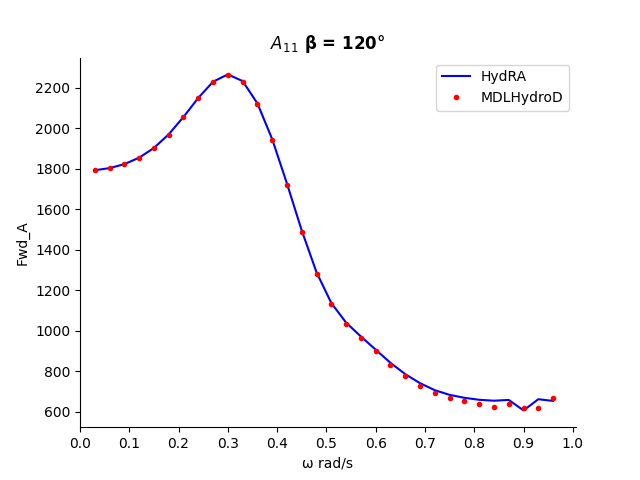
\includegraphics[width=\textwidth]{plots/kcs/added_mass_deg=120/a11.png}
        \caption{$A_{22} \, \beta = 120^{\circ}$}
    \end{subfigure}
    \begin{subfigure}[b]{0.45\textwidth}
        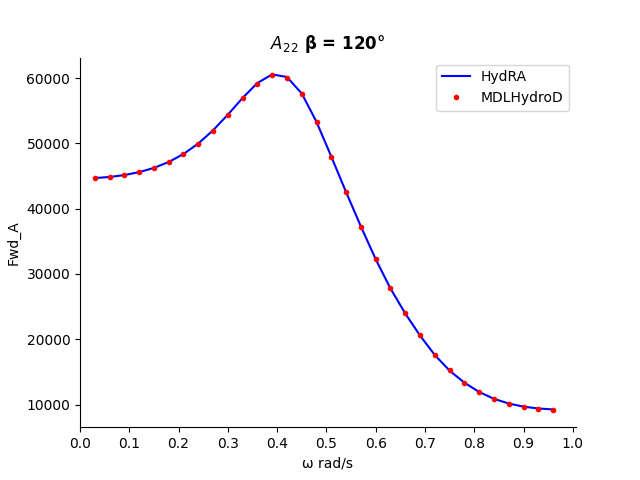
\includegraphics[width=\textwidth]{plots/kcs/added_mass_deg=120/a22.png}
        \caption{$A_{22} \, \beta = 120^{\circ}$}
    \end{subfigure}
    \vspace{5pt}%
    \begin{subfigure}[b]{0.45\textwidth}
        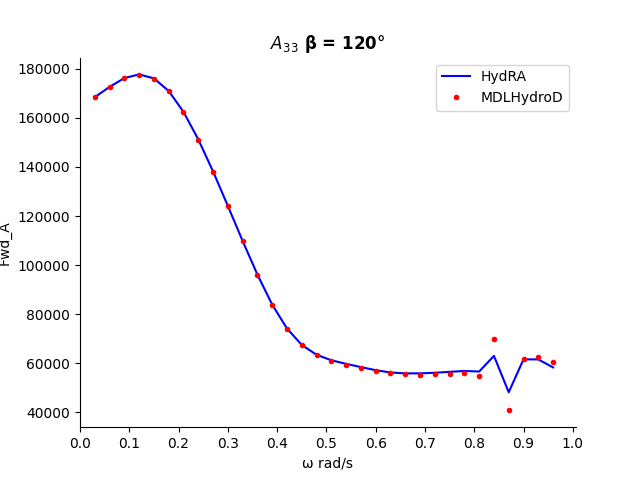
\includegraphics[width=\textwidth]{plots/kcs/added_mass_deg=120/a33.png}
        \caption{$A_{11}\, \beta = 120^{\circ}$}
    \end{subfigure}
    \begin{subfigure}[b]{0.45\textwidth}
        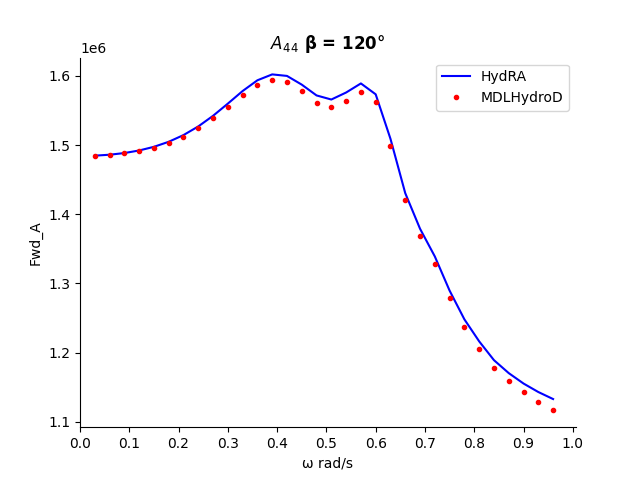
\includegraphics[width=\textwidth]{plots/kcs/added_mass_deg=120/a44.png}
        \caption{$A_{22} \, \beta = 120^{\circ}$}
    \end{subfigure}
    \vspace{5pt}%
    \begin{subfigure}[b]{0.45\textwidth}
        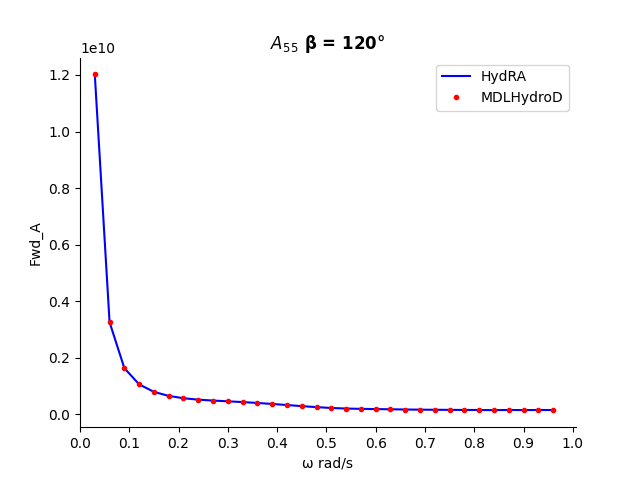
\includegraphics[width=\textwidth]{plots/kcs/added_mass_deg=120/a55.png}
        \caption{$A_{22} \, \beta = 120^{\circ}$}
    \end{subfigure}
    \begin{subfigure}[b]{0.45\textwidth}
        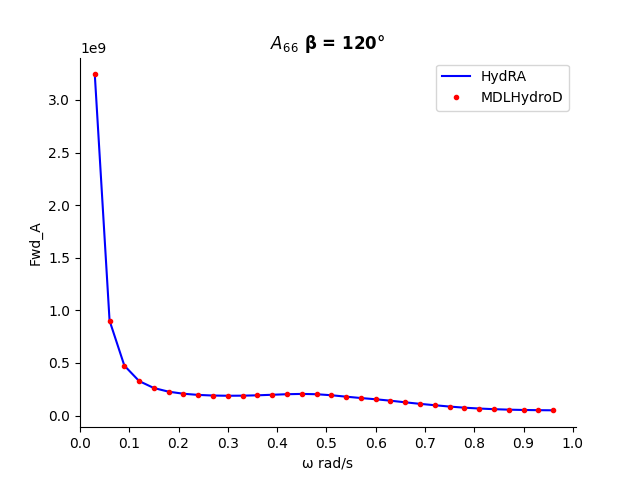
\includegraphics[width=\textwidth]{plots/kcs/added_mass_deg=120/a66.png}
        \caption{$A_{22} \, \beta = 120^{\circ}$}
    \end{subfigure}
    \caption{KCS vessel added mass comparison for degree $\beta=120^{\circ}$}
    \label{fig:kcs_addedmass_1}
\end{figure}

\subsection{Radiation Damping}
\begin{figure}[H]
    \centering
    \begin{subfigure}[b]{0.45\textwidth}
        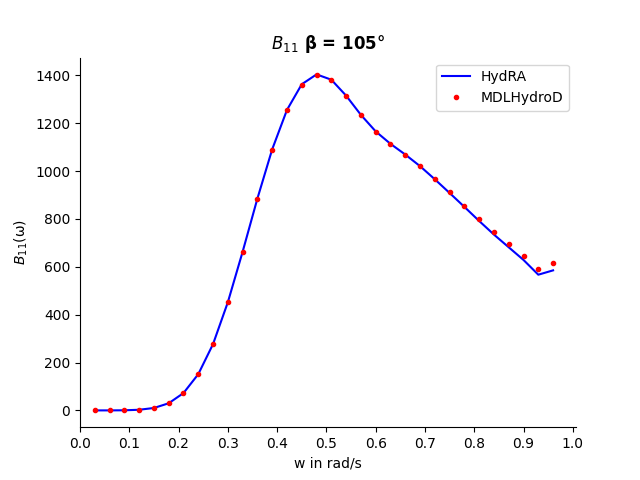
\includegraphics[width=\textwidth]{plots/kcs/rad_damp_deg_120/b11.png}
        \caption{$B_{11} \, \beta = 105^{\circ}$}
    \end{subfigure}
    \begin{subfigure}[b]{0.45\textwidth}
        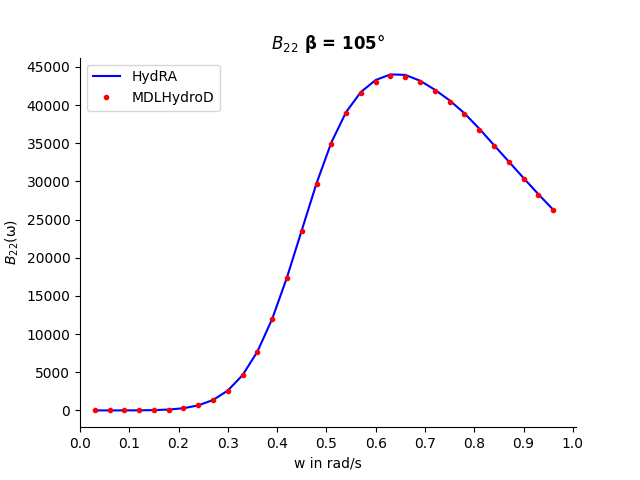
\includegraphics[width=\textwidth]{plots/kcs/rad_damp_deg_120/b22.png}
        \caption{$B_{22} \, \beta = 105^{\circ}$}
    \end{subfigure}
    \vspace{5pt}%
    \begin{subfigure}[b]{0.45\textwidth}
        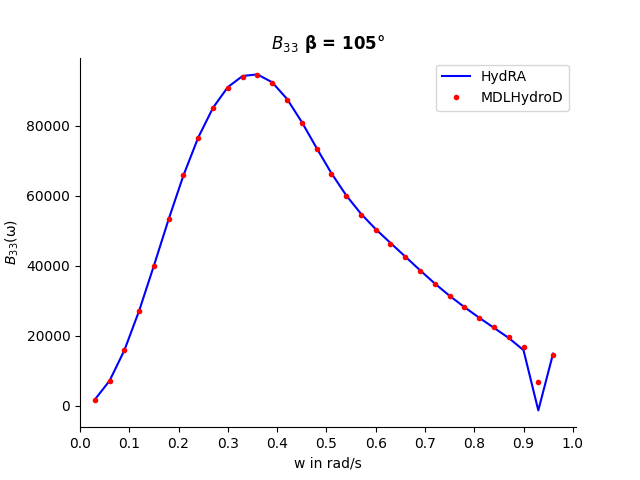
\includegraphics[width=\textwidth]{plots/kcs/rad_damp_deg_120/b33.png}
        \caption{$B_{33}\, \beta = 105^{\circ}$}
    \end{subfigure}
    \begin{subfigure}[b]{0.45\textwidth}
        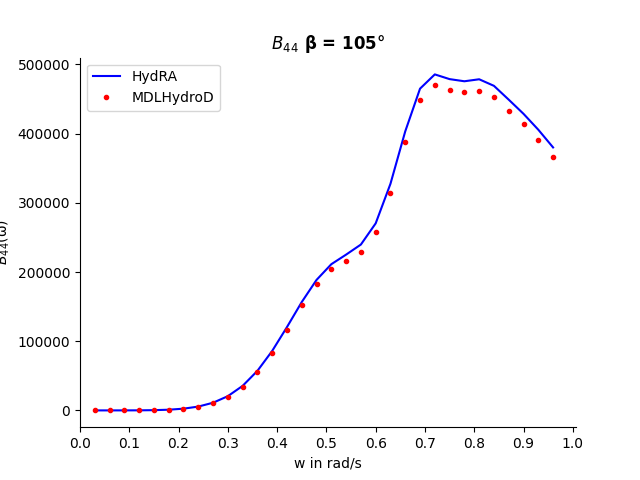
\includegraphics[width=\textwidth]{plots/kcs/rad_damp_deg_120/b44.png}
        \caption{$B_{44} \, \beta = 105^{\circ}$}
    \end{subfigure}
    \vspace{5pt}%
    \begin{subfigure}[b]{0.45\textwidth}
        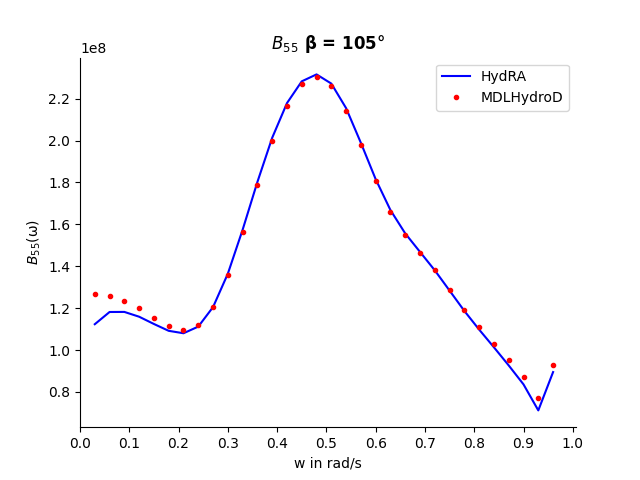
\includegraphics[width=\textwidth]{plots/kcs/rad_damp_deg_120/b55.png}
        \caption{$B_{55} \, \beta = 105^{\circ}$}
    \end{subfigure}
    \begin{subfigure}[b]{0.45\textwidth}
        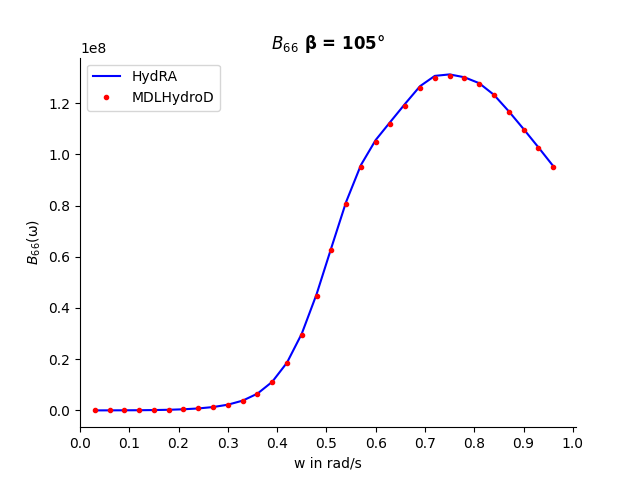
\includegraphics[width=\textwidth]{plots/kcs/rad_damp_deg_120/b66.png}
        \caption{$B_{66} \, \beta = 105^{\circ}$}
    \end{subfigure}
    \caption{KCS vessel radiation damping comparison for degree $\beta= 105^{\circ}$}
    \label{fig:radition_damp_125}
\end{figure}

\subsection{Froude Krylov Force}
\begin{figure}[H]
    \centering
    \begin{subfigure}[b]{0.45\textwidth}
        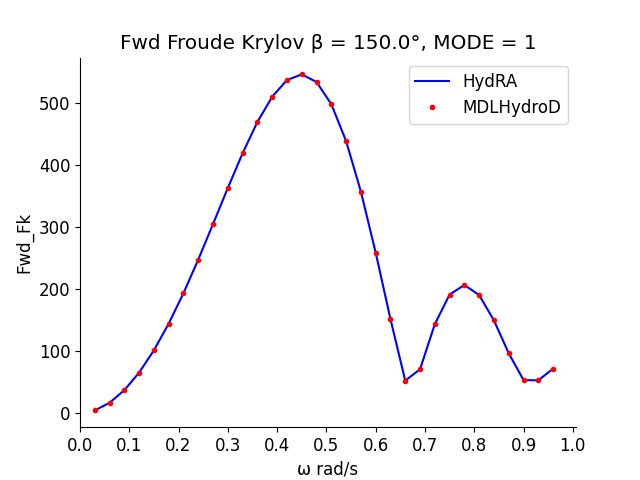
\includegraphics[width=\textwidth]{plots/kcs/fk/fk1.png}
        \caption{Surge FkFrc $\beta = 150^{\circ}$}
    \end{subfigure}
    \begin{subfigure}[b]{0.45\textwidth}
        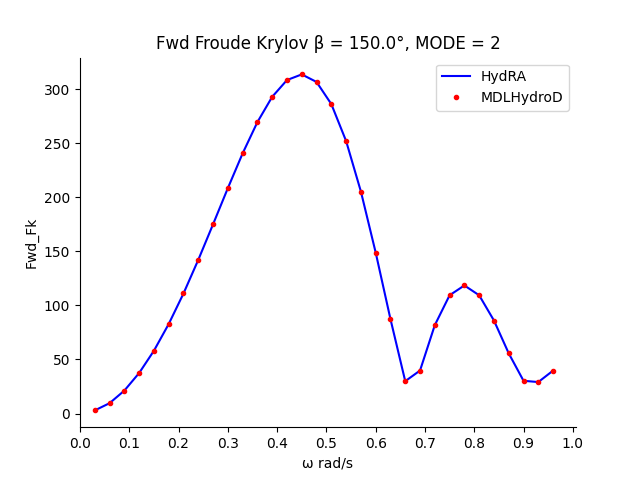
\includegraphics[width=\textwidth]{plots/kcs/fk/fk2.png}
        \caption{Sway FkFrc $\beta = 150^{\circ}$}
    \end{subfigure}
    \vspace{5pt}%
    \begin{subfigure}[b]{0.45\textwidth}
        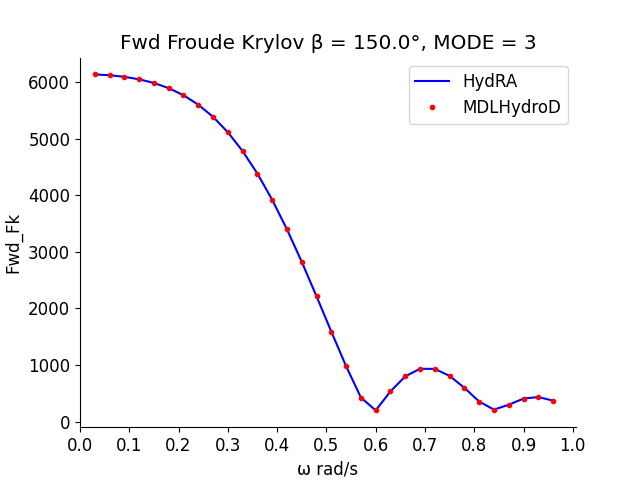
\includegraphics[width=\textwidth]{plots/kcs/fk/fk3.png}
        \caption{Heave FkFrc $\beta = 150^{\circ}$}
    \end{subfigure}
    \begin{subfigure}[b]{0.45\textwidth}
        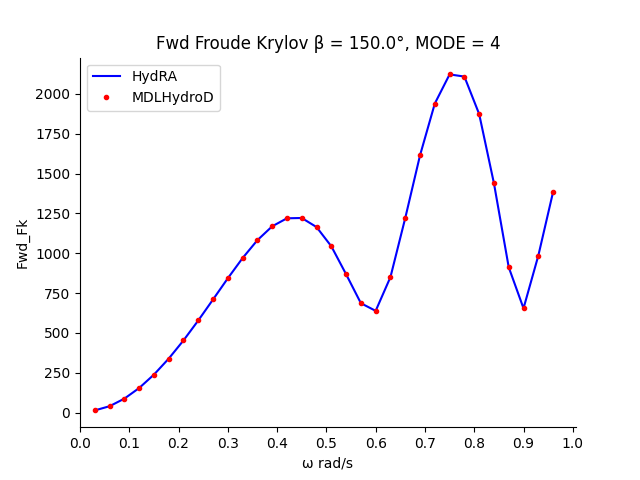
\includegraphics[width=\textwidth]{plots/kcs/fk/fk4.png}
        \caption{Roll FkFrc $\beta = 105^{\circ}$}
    \end{subfigure}
    \vspace{5pt}%
    \begin{subfigure}[b]{0.45\textwidth}
        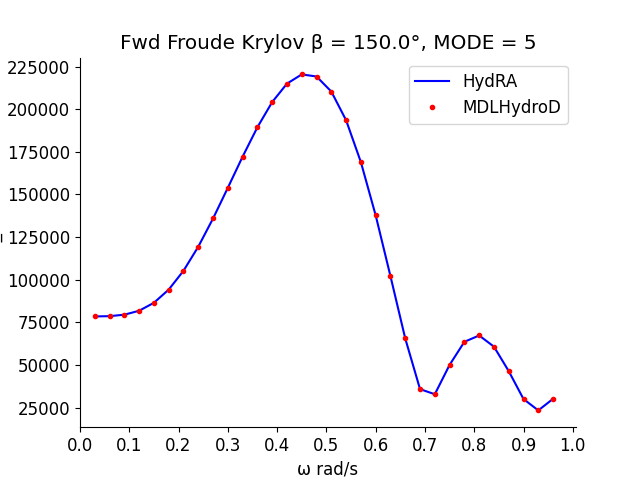
\includegraphics[width=\textwidth]{plots/kcs/fk/fk5.png}
        \caption{Pitch FkFrc $\beta = 105^{\circ}$}
    \end{subfigure}
    \begin{subfigure}[b]{0.45\textwidth}
        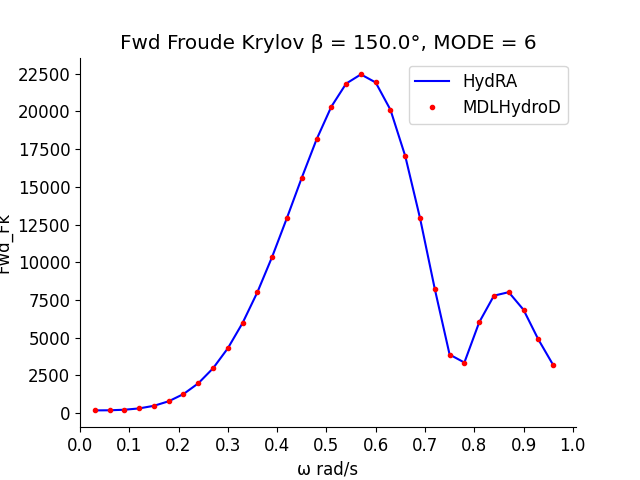
\includegraphics[width=\textwidth]{plots/kcs/fk/fk6.png}
        \caption{Yaw FkFrc $\beta = 105^{\circ}$}
    \end{subfigure}
    \caption{KCS vessel froude krylov force comparison for degree $\beta= 105^{\circ}$}
    \label{fig:kcs_froude_krylov}
\end{figure}

\subsection{Scattering Force}
\begin{figure}[H]
    \centering
    \begin{subfigure}[b]{0.45\textwidth}
        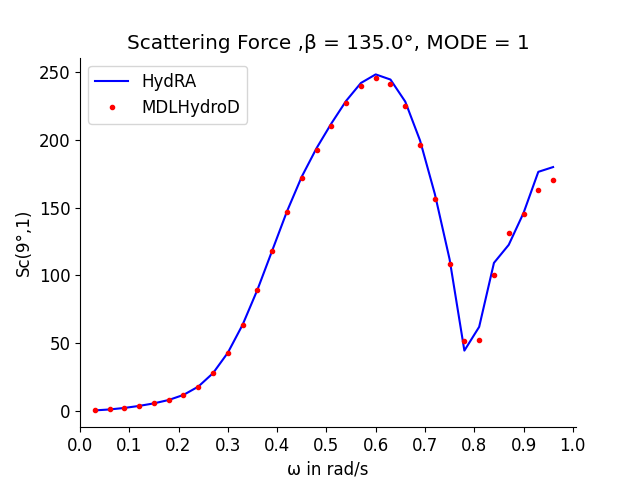
\includegraphics[width=\textwidth]{plots/kcs/sc/sc1.png}
        \caption{Surge ScFrc $\beta = 135^{\circ}$}
    \end{subfigure}
    \begin{subfigure}[b]{0.45\textwidth}
        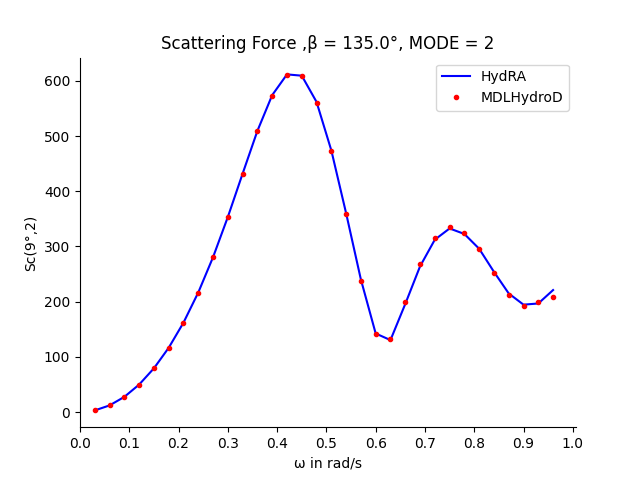
\includegraphics[width=\textwidth]{plots/kcs/sc/sc2.png}
        \caption{Sway ScFrc $\beta = 135^{\circ}$}
    \end{subfigure}
    \vspace{5pt}%
    \begin{subfigure}[b]{0.45\textwidth}
        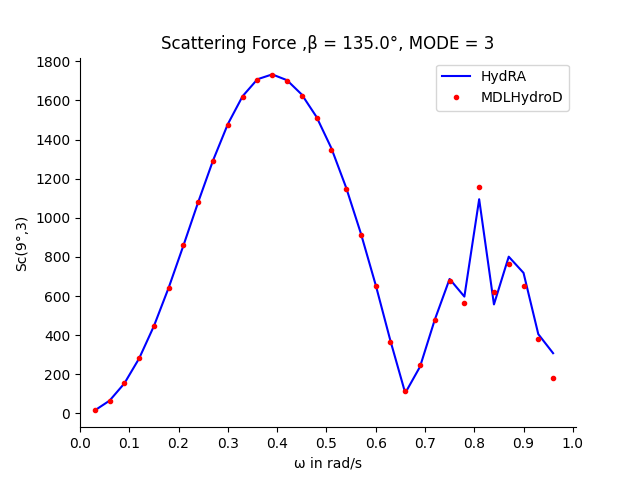
\includegraphics[width=\textwidth]{plots/kcs/sc/sc3.png}
        \caption{Heave ScFrc $\beta = 135^{\circ}$}
    \end{subfigure}
    \begin{subfigure}[b]{0.45\textwidth}
        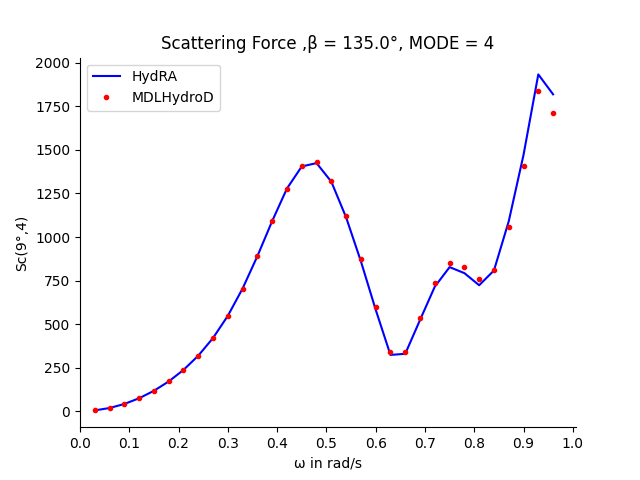
\includegraphics[width=\textwidth]{plots/kcs/sc/sc4.png}
        \caption{Roll ScFrc $\beta = 105^{\circ}$}
    \end{subfigure}
    \vspace{5pt}%
    \begin{subfigure}[b]{0.45\textwidth}
        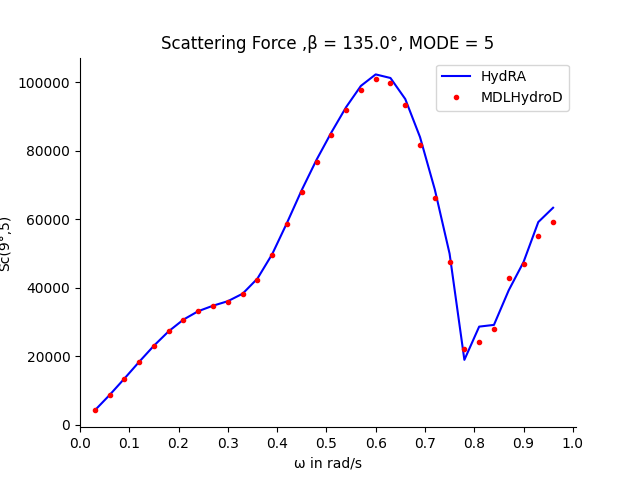
\includegraphics[width=\textwidth]{plots/kcs/sc/sc5.png}
        \caption{Pitch ScFrc $\beta = 105^{\circ}$}
    \end{subfigure}
    \begin{subfigure}[b]{0.45\textwidth}
        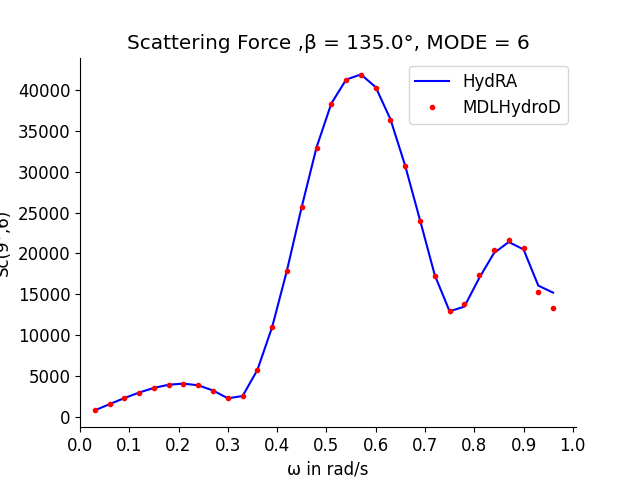
\includegraphics[width=\textwidth]{plots/kcs/sc/sc6.png}
        \caption{Yaw ScFrc $\beta = 105^{\circ}$}
    \end{subfigure}
    \caption{KCS vessel Scattering force comparison for degree $\beta= 135^{\circ}$}
    \label{fig:kcs_scattering_135}
\end{figure}

\subsection{RAO}
\begin{figure}[H]
    \centering
    \begin{subfigure}[b]{0.45\textwidth}
        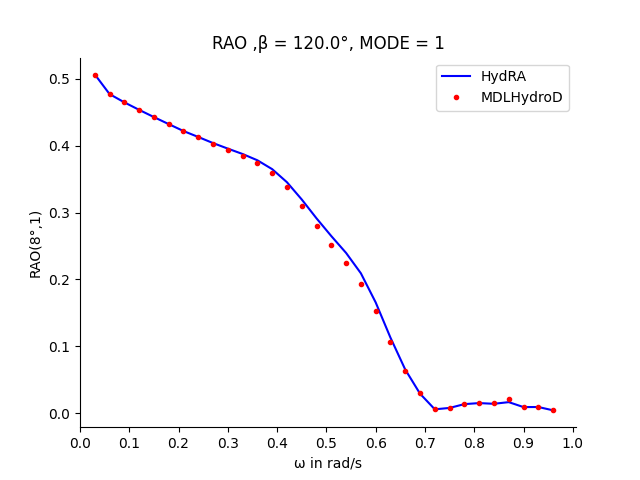
\includegraphics[width=\textwidth]{plots/kcs/rao/rao1.png}
        \caption{Surge RAO $\beta = 120^{\circ}$}
    \end{subfigure}
    \begin{subfigure}[b]{0.45\textwidth}
        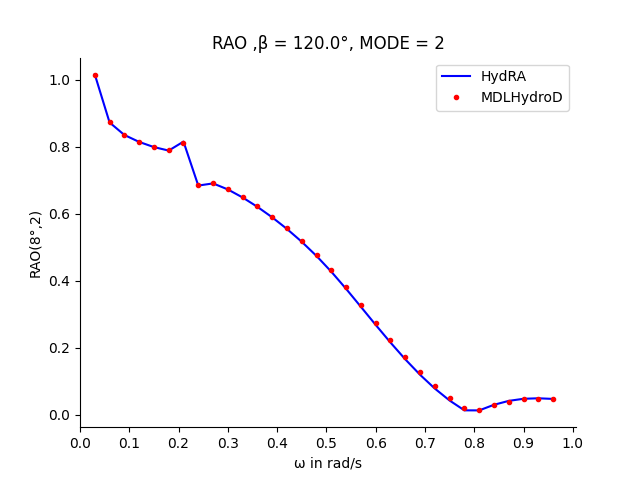
\includegraphics[width=\textwidth]{plots/kcs/rao/rao2.png}
        \caption{Sway RAO $\beta = 120^{\circ}$}
    \end{subfigure}
    \vspace{5pt}%
    \begin{subfigure}[b]{0.45\textwidth}
        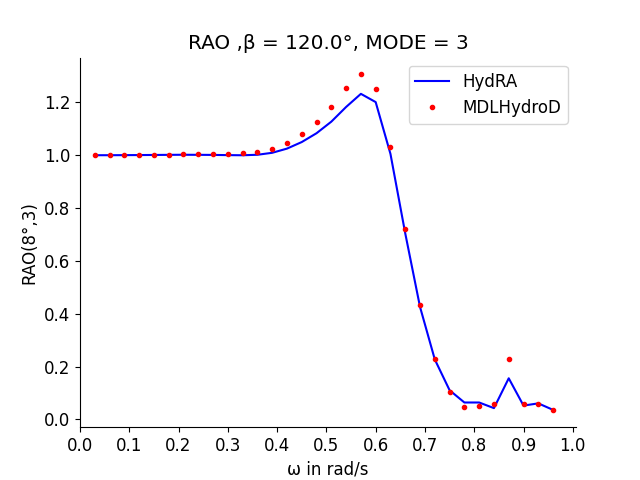
\includegraphics[width=\textwidth]{plots/kcs/rao/rao3.png}
        \caption{Heave RAO $\beta = 120^{\circ}$}
    \end{subfigure}
    \begin{subfigure}[b]{0.45\textwidth}
        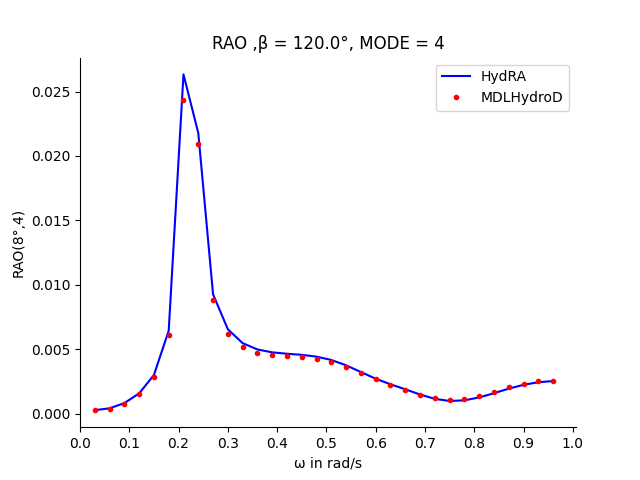
\includegraphics[width=\textwidth]{plots/kcs/rao/rao4.png}
        \caption{Roll RAO $\beta = 120^{\circ}$}
    \end{subfigure}
    \vspace{5pt}%
    \begin{subfigure}[b]{0.45\textwidth}
        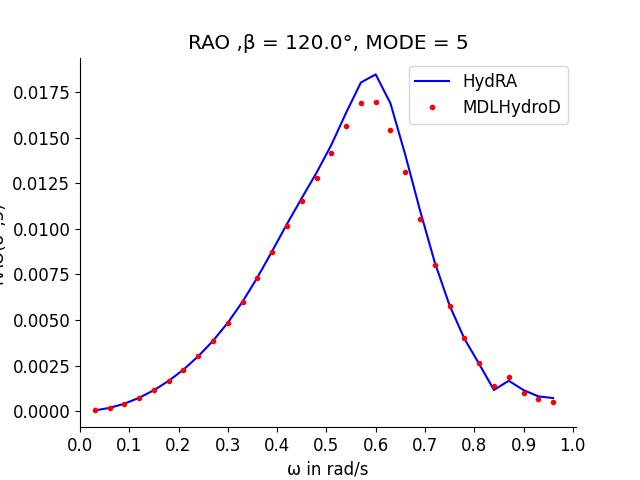
\includegraphics[width=\textwidth]{plots/kcs/rao/rao5.png}
        \caption{Pitch RAO $\beta = 120^{\circ}$}
    \end{subfigure}
    \begin{subfigure}[b]{0.45\textwidth}
        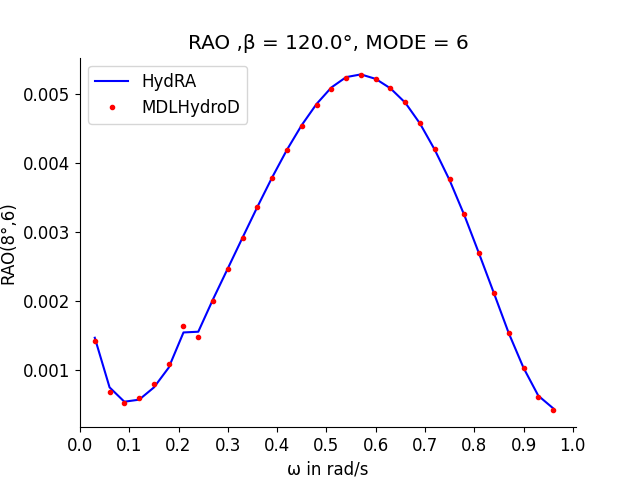
\includegraphics[width=\textwidth]{plots/kcs/rao/rao6.png}
        \caption{Yaw RAO $\beta = 120^{\circ}$}
    \end{subfigure}
    \caption{KCS vessel RAO comparison for degree $\beta= 120^{\circ}$}
    \label{fig:kcs_rao_120}
\end{figure}
\newpage
\begin{figure}[H]
    \centering
    \begin{subfigure}[b]{0.45\textwidth}
        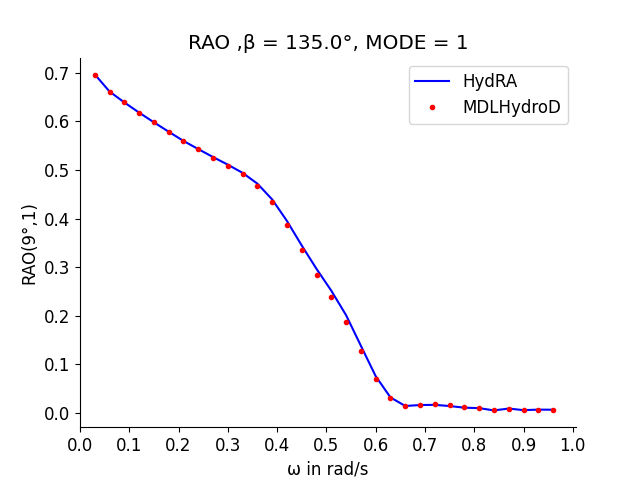
\includegraphics[width=\textwidth]{plots/kcs/rao2/rao1.png}
        \caption{Surge RAO $\beta = 135^{\circ}$}
    \end{subfigure}
    \begin{subfigure}[b]{0.45\textwidth}
        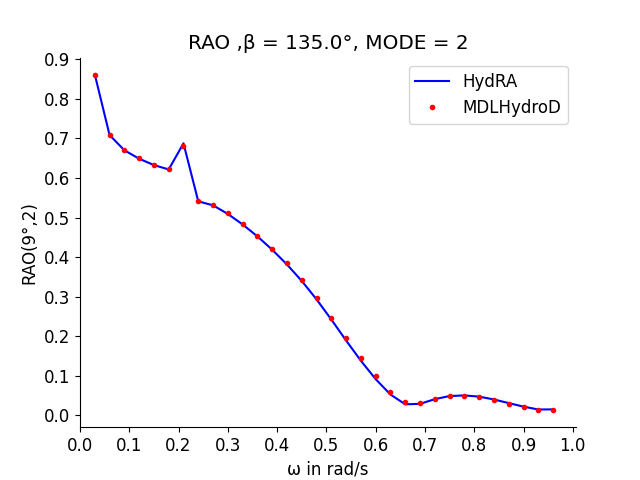
\includegraphics[width=\textwidth]{plots/kcs/rao2/rao2.png}
        \caption{Sway RAO $\beta = 135^{\circ}$}
    \end{subfigure}
    \vspace{5pt}%
    \begin{subfigure}[b]{0.45\textwidth}
        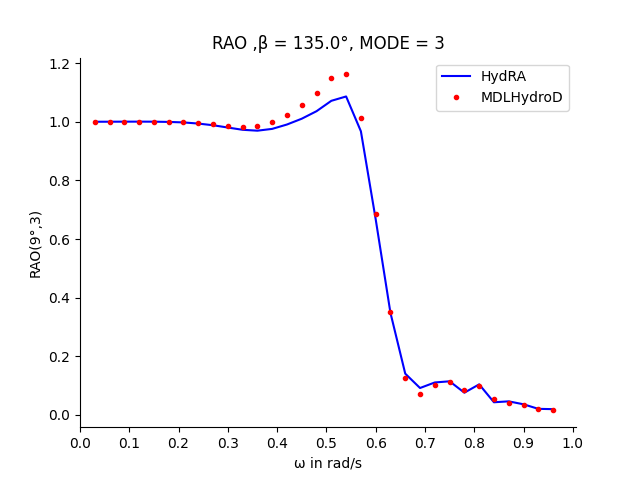
\includegraphics[width=\textwidth]{plots/kcs/rao2/rao3.png}
        \caption{Heave RAO $\beta = 135^{\circ}$}
    \end{subfigure}
    \begin{subfigure}[b]{0.45\textwidth}
        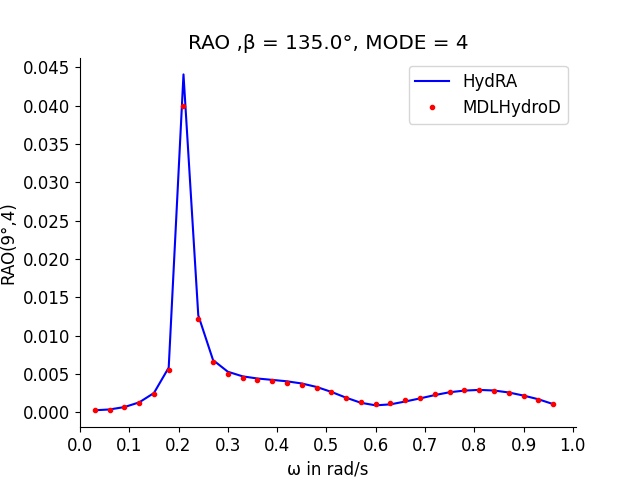
\includegraphics[width=\textwidth]{plots/kcs/rao2/rao4.png}
        \caption{Roll RAO $\beta = 135^{\circ}$}
    \end{subfigure}
    \vspace{5pt}%
    \begin{subfigure}[b]{0.45\textwidth}
        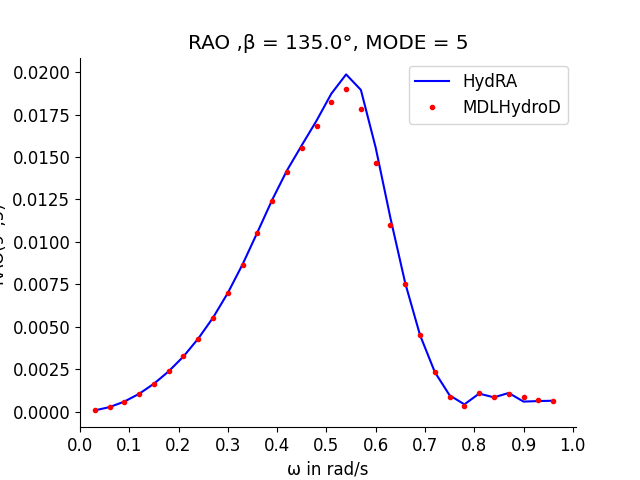
\includegraphics[width=\textwidth]{plots/kcs/rao2/rao5.png}
        \caption{Pitch RAO $\beta = 135^{\circ}$}
    \end{subfigure}
    \begin{subfigure}[b]{0.45\textwidth}
        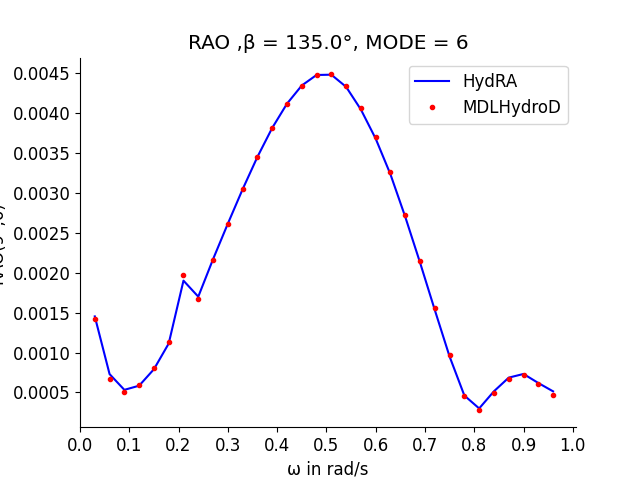
\includegraphics[width=\textwidth]{plots/kcs/rao2/rao6.png}
        \caption{Yaw RAO $\beta = 135^{\circ}$}
    \end{subfigure}
    \caption{KCS vessel RAO comparison for degree $\beta= 135^{\circ}$}
    \label{fig:kcs_rao_135}
\end{figure}


\newpage
\section{Forward speed comparisons for KVLCC Vessel}
Principle perticulars for KVLCC2 (Oil tanker) are given in the table \ref{tab:kvlcc2_particulars}.
For comparison, frequencies are used from
$-0.03$ with $+0.03$ increment and in totoal $34$ frequencies are used. Ship's speed is $8\,\si{m.s^{-1}}$. 
Incident angles used 
ranges from $0^{\circ}$ to $345^{\circ}$ with $15^{\circ}$ increment. Simulation is ran for all 6 modes of motion.  
The comparison of added mass for different angles are shown in figure \ref{fig:kvlcc_addedmass}.
Comparisons of radiation damping is shown in figure \ref{fig:kvlcc_radition_damp_105}. 
Comparisons of Froude Krylov force is shown in figure \ref{fig:kvlcc_froude_krylov}.
Comparisons of Scattering force is shown in figure \ref{fig:kvlcc_scattering}. 
Comparisons of RAO is shown in figure \ref{fig:kcs_rao_120}
and figure \ref{fig:kvlcc_rao_135}
\\[1.5cm]

\begin{table}[h]
    \centering{%
    \setlength{\tabcolsep}{10pt} % Default value: 6pt
    \renewcommand{\arraystretch}{1.17} % Default value: 1
    \begin{tabular}{{|c|c|}}
    \hline
    Main Particulars & Value\\
    \hline
    Length between perpendiculars $L ~(m)$ & 320  \\ 
    Breadth $B ~(m)$ & 58  \\
    Draft $d ~(m)$ & 20.8  \\
    Displacement $\nabla ~(m^{3})$ & 312622  \\
    Block coefficient $C_{b}$ & 0.8098   \\
    Radius of Gyration $R_{zz}/L$ & 0.25 \\
    Metacentric height $GM ~(m)$ & 5.71 \\
    LCB (\% of $L$ from midship, forward +ve) & 3.48\% \\
    Forward speed & 8.00 $\si{ms^{-1}}$ \\
    \hline
    \end{tabular}
    }
    \caption{$\text{KVLCC2 principal particulars}$}
    \label{tab:kvlcc2_particulars}
\end{table}
\subsection{Added Mass}
\begin{figure}[H]
    \centering
    \begin{subfigure}[b]{0.45\textwidth}
        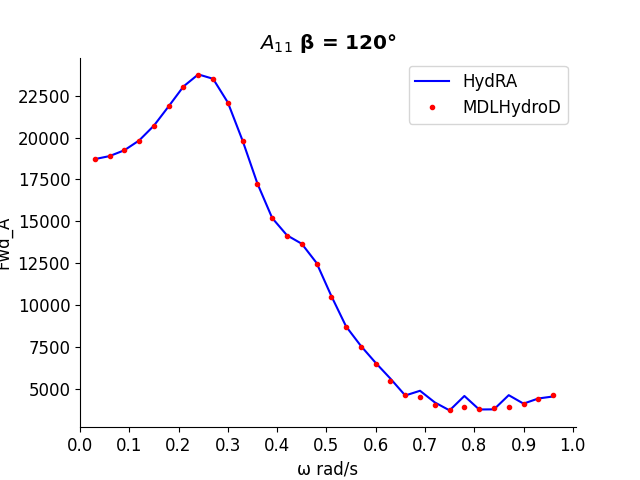
\includegraphics[width=\textwidth]{plots/kvlcc/added_mass/a11.png}
        \caption{$A_{22} \, \beta = 120^{\circ}$}
    \end{subfigure}
    \begin{subfigure}[b]{0.45\textwidth}
        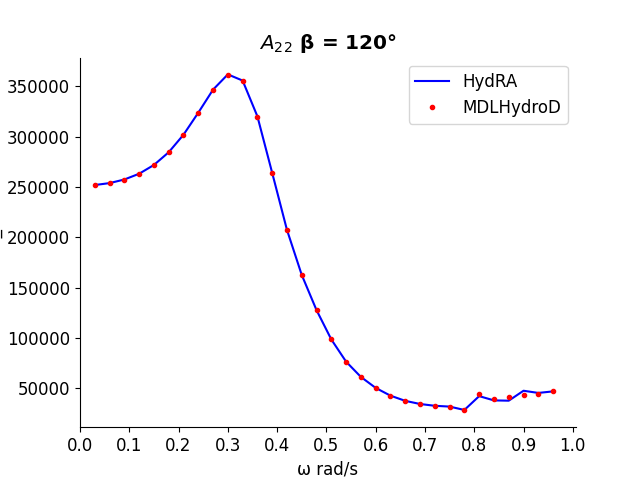
\includegraphics[width=\textwidth]{plots/kvlcc/added_mass/a22.png}
        \caption{$A_{22} \, \beta = 120^{\circ}$}
    \end{subfigure}
    \vspace{5pt}%
    \begin{subfigure}[b]{0.45\textwidth}
        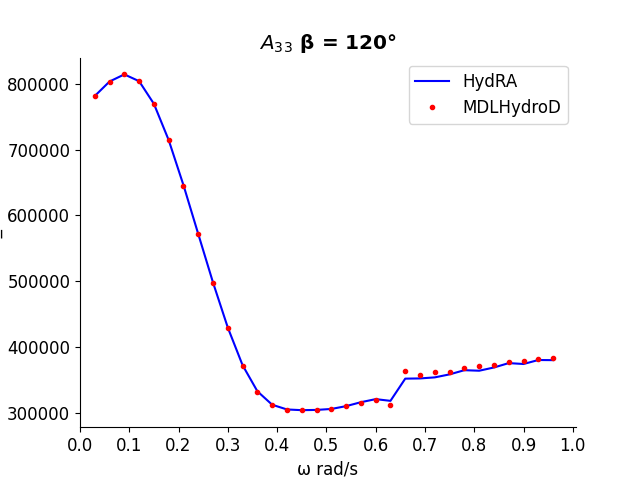
\includegraphics[width=\textwidth]{plots/kvlcc/added_mass/a33.png}
        \caption{$A_{11}\, \beta = 120^{\circ}$}
    \end{subfigure}
    \begin{subfigure}[b]{0.45\textwidth}
        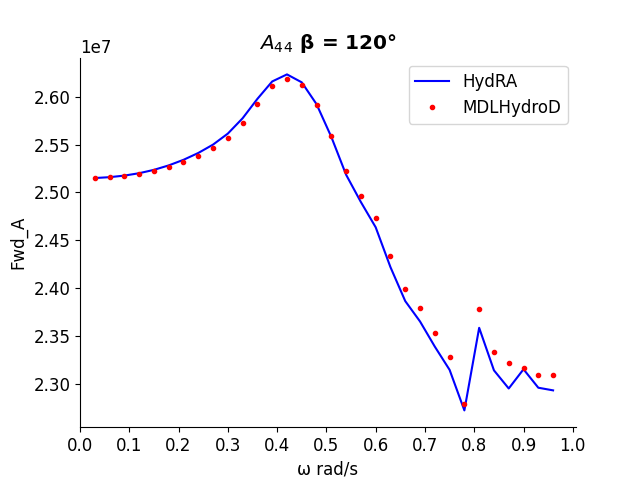
\includegraphics[width=\textwidth]{plots/kvlcc/added_mass/a44.png}
        \caption{$A_{22} \, \beta = 120^{\circ}$}
    \end{subfigure}
    \vspace{5pt}%
    \begin{subfigure}[b]{0.45\textwidth}
        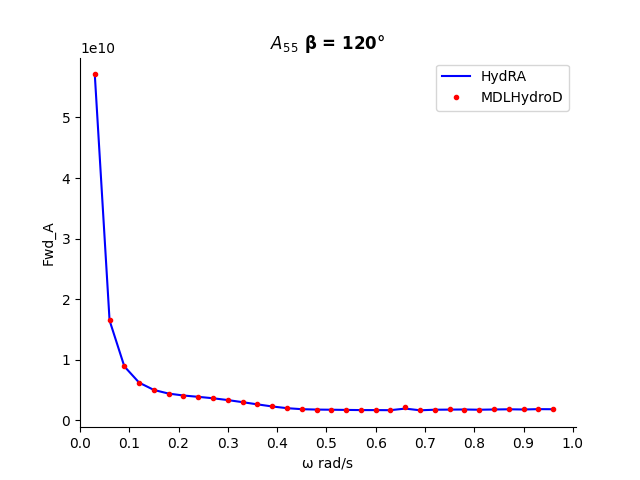
\includegraphics[width=\textwidth]{plots/kvlcc/added_mass/a55.png}
        \caption{$A_{22} \, \beta = 120^{\circ}$}
    \end{subfigure}
    \begin{subfigure}[b]{0.45\textwidth}
        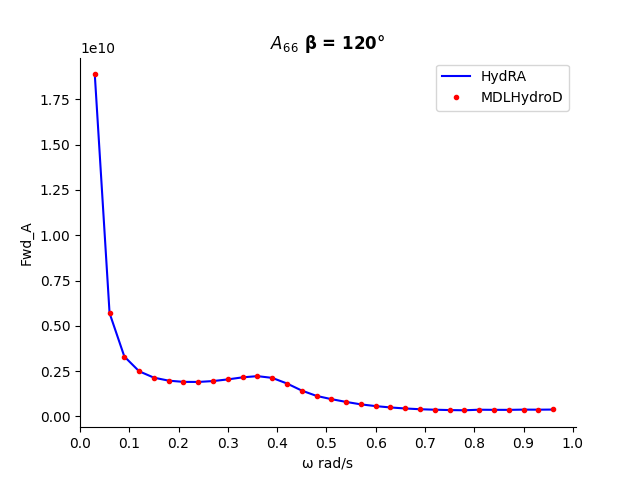
\includegraphics[width=\textwidth]{plots/kvlcc/added_mass/a66.png}
        \caption{$A_{22} \, \beta = 120^{\circ}$}
    \end{subfigure}
    \caption{KCS vessel added mass comparison for $\beta=120^{\circ}$}
    \label{fig:kvlcc_addedmass}
\end{figure}

\subsection{Radiation Damping}
\begin{figure}[H]
    \centering
    \begin{subfigure}[b]{0.45\textwidth}
        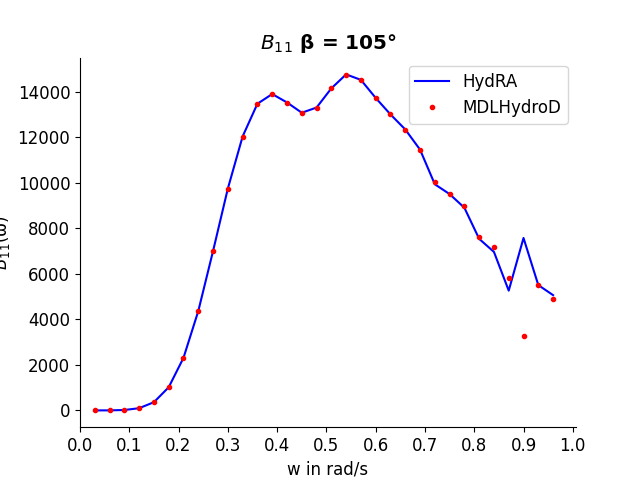
\includegraphics[width=\textwidth]{plots/kvlcc/radiation_damp/b11.png}
        \caption{$B_{11} \, \beta = 105^{\circ}$}
    \end{subfigure}
    \begin{subfigure}[b]{0.45\textwidth}
        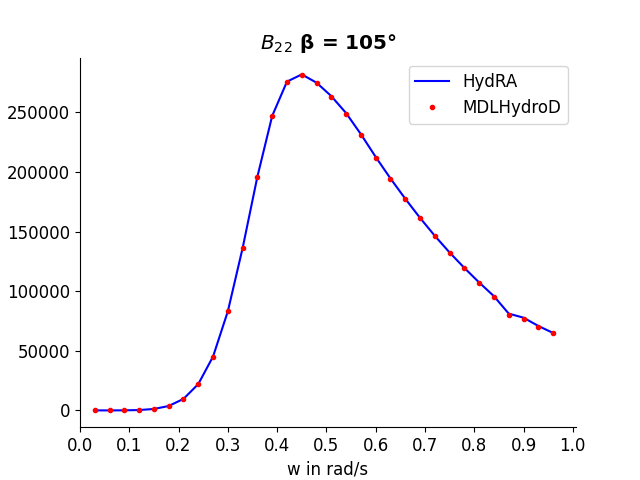
\includegraphics[width=\textwidth]{plots/kvlcc/radiation_damp/b22.png}
        \caption{$B_{22} \, \beta = 105^{\circ}$}
    \end{subfigure}
    \vspace{5pt}%
    \begin{subfigure}[b]{0.45\textwidth}
        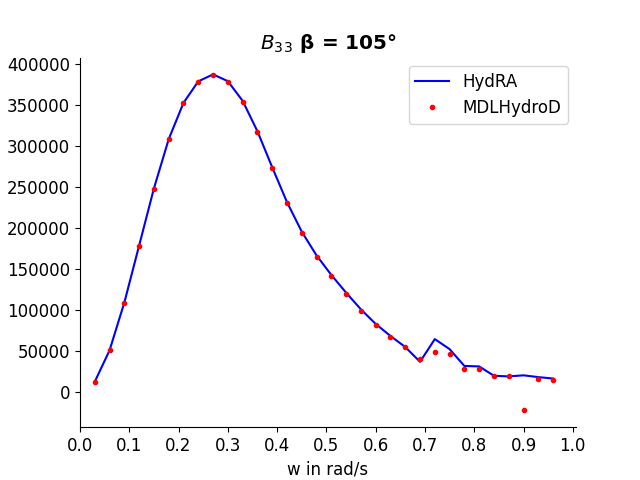
\includegraphics[width=\textwidth]{plots/kvlcc/radiation_damp/b33.png}
        \caption{$B_{33}\, \beta = 105^{\circ}$}
    \end{subfigure}
    \begin{subfigure}[b]{0.45\textwidth}
        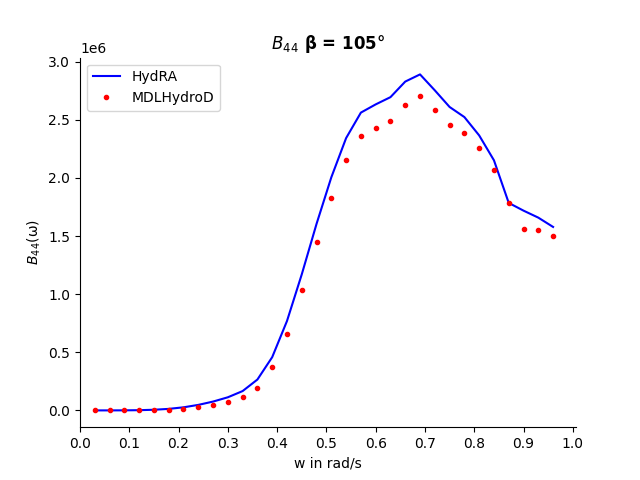
\includegraphics[width=\textwidth]{plots/kvlcc/radiation_damp/b44.png}
        \caption{$B_{44} \, \beta = 105^{\circ}$}
    \end{subfigure}
    \vspace{5pt}%
    \begin{subfigure}[b]{0.45\textwidth}
        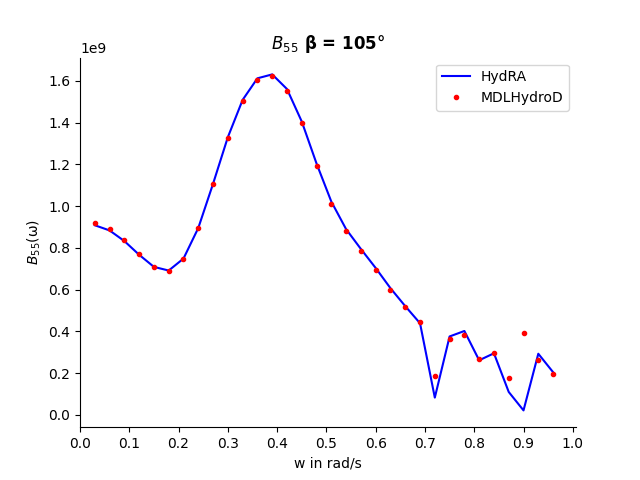
\includegraphics[width=\textwidth]{plots/kvlcc/radiation_damp/b55.png}
        \caption{$B_{55} \, \beta = 105^{\circ}$}
    \end{subfigure}
    \begin{subfigure}[b]{0.45\textwidth}
        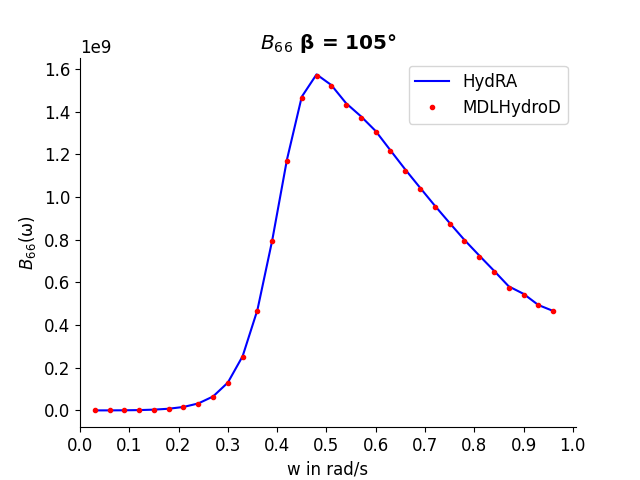
\includegraphics[width=\textwidth]{plots/kvlcc/radiation_damp/b66.png}
        \caption{$B_{66} \, \beta = 105^{\circ}$}
    \end{subfigure}
    \caption{KVLCC2 vessel radiation damping comparison for $\beta= 105^{\circ}$}
    \label{fig:kvlcc_radition_damp_105}
\end{figure}

\subsection{Froude Krylov Force}
\begin{figure}[H]
    \centering
    \begin{subfigure}[b]{0.45\textwidth}
        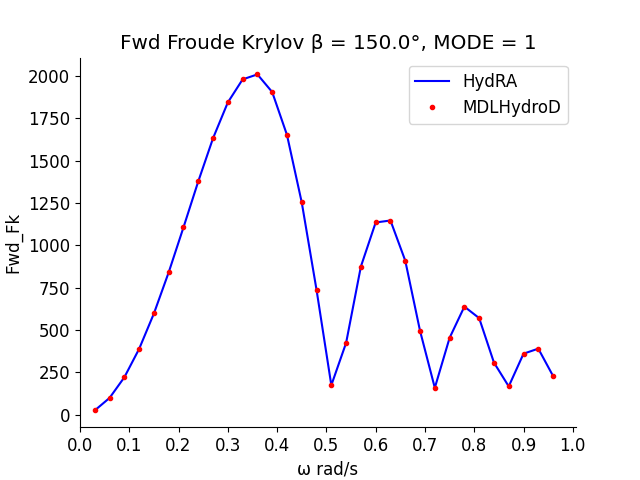
\includegraphics[width=\textwidth]{plots/kvlcc/fk/fk1.png}
        \caption{$Fk \, \beta = 150^{\circ}$}
    \end{subfigure}
    \begin{subfigure}[b]{0.45\textwidth}
        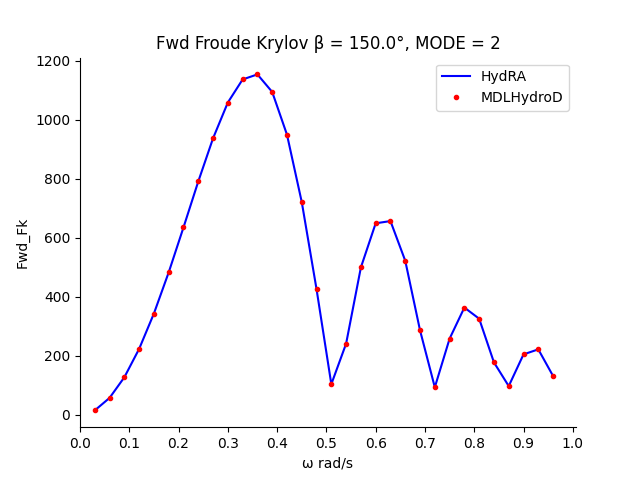
\includegraphics[width=\textwidth]{plots/kvlcc/fk/fk2.png}
        \caption{$Fk \, \beta = 150^{\circ}$}
    \end{subfigure}
    \vspace{5pt}%
    \begin{subfigure}[b]{0.45\textwidth}
        \includegraphics[width=\textwidth]{plots/kvlcc/fk/fk3.png}
        \caption{$Fk \, \beta = 150^{\circ}$}
    \end{subfigure}
    \begin{subfigure}[b]{0.45\textwidth}
        \includegraphics[width=\textwidth]{plots/kvlcc/fk/fk4.png}
        \caption{$Fk \, \beta = 150^{\circ}$}
    \end{subfigure}
    \vspace{5pt}%
    \begin{subfigure}[b]{0.45\textwidth}
        \includegraphics[width=\textwidth]{plots/kvlcc/fk/fk5.png}
        \caption{$Fk \, \beta = 150^{\circ}$}
    \end{subfigure}
    \begin{subfigure}[b]{0.45\textwidth}
        \includegraphics[width=\textwidth]{plots/kvlcc/fk/fk6.png}
        \caption{$Fk \, \beta = 150^{\circ}$}
    \end{subfigure}
    \caption{KVLCC2 vessel froude krylov force comparison for $\beta= 150^{\circ}$}
    \label{fig:kvlcc_froude_krylov}
\end{figure}

\subsection{Scattering Force}
\begin{figure}[H]
    \centering
    \begin{subfigure}[b]{0.45\textwidth}
        \includegraphics[width=\textwidth]{plots/kvlcc/sc/sc1.png}
        \caption{Surge ScFrc $\beta = 135^{\circ}$}
    \end{subfigure}
    \begin{subfigure}[b]{0.45\textwidth}
        \includegraphics[width=\textwidth]{plots/kvlcc/sc/sc2.png}
        \caption{Sway ScFrc $\beta = 135^{\circ}$}
    \end{subfigure}
    \vspace{5pt}%
    \begin{subfigure}[b]{0.45\textwidth}
        \includegraphics[width=\textwidth]{plots/kvlcc/sc/sc3.png}
        \caption{Heave ScFrc $\beta = 135^{\circ}$}
    \end{subfigure}
    \begin{subfigure}[b]{0.45\textwidth}
        \includegraphics[width=\textwidth]{plots/kvlcc/sc/sc4.png}
        \caption{Roll ScFrc $\beta = 135^{\circ}$}
    \end{subfigure}
    \vspace{5pt}%
    \begin{subfigure}[b]{0.45\textwidth}
        \includegraphics[width=\textwidth]{plots/kvlcc/sc/sc5.png}
        \caption{Pitch ScFrc $\beta = 135^{\circ}$}
    \end{subfigure}
    \begin{subfigure}[b]{0.45\textwidth}
        \includegraphics[width=\textwidth]{plots/kvlcc/sc/sc6.png}
        \caption{Yaw ScFrc $\beta = 135^{\circ}$}
    \end{subfigure}
    \caption{KVLCC2 vessel Scattering force comparison for $\beta= 135^{\circ}$}
    \label{fig:kvlcc_scattering}
\end{figure}
\subsection{RAO}
\begin{figure}[H]
    \centering
    \begin{subfigure}[b]{0.45\textwidth}
        \includegraphics[width=\textwidth]{plots/kcs/rao/rao1.png}
        \caption{Surge RAO $\beta = 120^{\circ}$}
    \end{subfigure}
    \begin{subfigure}[b]{0.45\textwidth}
        \includegraphics[width=\textwidth]{plots/kcs/rao/rao2.png}
        \caption{Sway RAO $\beta = 120^{\circ}$}
    \end{subfigure}
    \vspace{5pt}%
    \begin{subfigure}[b]{0.45\textwidth}
        \includegraphics[width=\textwidth]{plots/kcs/rao/rao3.png}
        \caption{Heave RAO $\beta = 120^{\circ}$}
    \end{subfigure}
    \begin{subfigure}[b]{0.45\textwidth}
        \includegraphics[width=\textwidth]{plots/kcs/rao/rao4.png}
        \caption{Roll RAO $\beta = 120^{\circ}$}
    \end{subfigure}
    \vspace{5pt}%
    \begin{subfigure}[b]{0.45\textwidth}
        \includegraphics[width=\textwidth]{plots/kcs/rao/rao5.png}
        \caption{Pitch RAO $\beta = 120^{\circ}$}
    \end{subfigure}
    \begin{subfigure}[b]{0.45\textwidth}
        \includegraphics[width=\textwidth]{plots/kcs/rao/rao6.png}
        \caption{Yaw RAO $\beta = 120^{\circ}$}
    \end{subfigure}
    \caption{KCS vessel RAO comparison for $\beta = 120^{\circ}$}
    \label{fig:kvlcc_rao_120}
\end{figure}
\begin{figure}[H]
    \centering
    \begin{subfigure}[b]{0.45\textwidth}
        \includegraphics[width=\textwidth]{plots/kcs/rao2/rao1.png}
        \caption{Surge RAO $\beta = 135^{\circ}$}
    \end{subfigure}
    \begin{subfigure}[b]{0.45\textwidth}
        \includegraphics[width=\textwidth]{plots/kcs/rao2/rao2.png}
        \caption{Sway RAO $\beta = 135^{\circ}$}
    \end{subfigure}
    \vspace{5pt}%
    \begin{subfigure}[b]{0.45\textwidth}
        \includegraphics[width=\textwidth]{plots/kcs/rao2/rao3.png}
        \caption{Heave RAO $\beta = 135^{\circ}$}
    \end{subfigure}
    \begin{subfigure}[b]{0.45\textwidth}
        \includegraphics[width=\textwidth]{plots/kcs/rao2/rao4.png}
        \caption{Roll RAO $\beta = 135^{\circ}$}
    \end{subfigure}
    \vspace{5pt}%
    \begin{subfigure}[b]{0.45\textwidth}
        \includegraphics[width=\textwidth]{plots/kcs/rao2/rao5.png}
        \caption{Pitch RAO $\beta = 135^{\circ}$}
    \end{subfigure}
    \begin{subfigure}[b]{0.45\textwidth}
        \includegraphics[width=\textwidth]{plots/kcs/rao2/rao6.png}
        \caption{Yaw RAO $\beta = 135^{\circ}$}
    \end{subfigure}
    \caption{KVLCC vessel RAO comparison for $\beta= 135^{\circ}$}
    \label{fig:kvlcc_rao_135}
\end{figure}

\newpage
\section{Drift force comparisons}
\label{sec:drift_frc}
Generally, in resistance prediction methods, the influence of the hull emergence 
angle is often disregarded or ignored. While far-field methods are believed to be 
unaffected by minor variations in the hull shape, near-field methods factor 
in the relative wave amplitude across the waterline to calculate the added 
resistance. Effect of hull emergence is explained in detail in \cite{guha2015effect}.
  After, incorporating the effect of hull emergence angle the actual 
value of Mean drift force is found lessor. This effect is shown in the below 
comparisons with WAMIT6. WAMIT6 does not consider hull emergence angle. Comparisons are done for 
KCS vessel, whose principal parameters are give in table (\ref{tab:kcs_principal_particulars}). 
The input parameters are same as used for forward speed comparisons.
\begin{figure}[H]
    \centering
    \begin{subfigure}[b]{0.45\textwidth}
        \includegraphics[width=\textwidth]{plots/kcs/drift/DrtFrc_12MODE_1.png}
        \caption{Surge drift force $\beta = 135^{\circ}$}
    \end{subfigure}
    \begin{subfigure}[b]{0.45\textwidth}
        \includegraphics[width=\textwidth]{plots/kcs/drift/DrtFrc_12MODE_2.png}
        \caption{Sway drift force $\beta = 135^{\circ}$}
    \end{subfigure}
    \vspace{5pt}%
    \begin{subfigure}[b]{0.45\textwidth}
        \includegraphics[width=\textwidth]{plots/kcs/drift/DrtFrc_12MODE_3.png}
        \caption{Heave drift force $\beta = 135^{\circ}$}
    \end{subfigure}
    \begin{subfigure}[b]{0.45\textwidth}
        \includegraphics[width=\textwidth]{plots/kcs/drift/DrtFrc_12MODE_4.png}
        \caption{Roll drift force $\beta = 135^{\circ}$}
    \end{subfigure}
    \vspace{5pt}%
    \caption{KCS vessel Drift force-I comparison for $\beta= 135^{\circ}$}
    \label{fig:kcs_drift_135_1}
\end{figure}

\begin{figure}[H]
    \centering
    \begin{subfigure}[b]{0.45\textwidth}
        \includegraphics[width=\textwidth]{plots/kcs/drift/DrtFrc_12MODE_5.png}
        \caption{Pitch drift force $\beta = 135^{\circ}$}
    \end{subfigure}
    \begin{subfigure}[b]{0.45\textwidth}
        \includegraphics[width=\textwidth]{plots/kcs/drift/DrtFrc_12MODE_6.png}
        \caption{Yaw drift force $\beta = 135^{\circ}$}
    \end{subfigure}
    \caption{KCS vessel Drift force-II comparison for $\beta= 135^{\circ}$}
    \label{fig:kcs_drift_135_2}
\end{figure}
